\documentclass[tikz,border=10pt]{standalone}
\begin{document}
		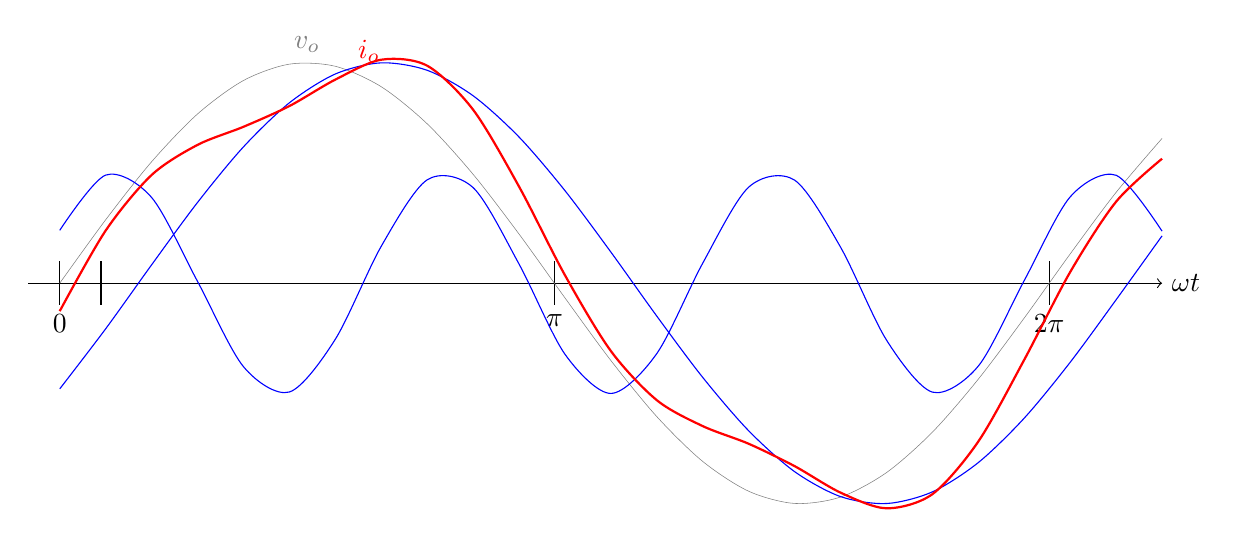
\begin{tikzpicture}
		\begin{scope}[xscale=2,yscale=2.8]
		\newcommand{\trig}{15 * pi / 180}
		\newcommand{\cutoff}{180 * pi / 180}
		\newcommand{\chargeend}{90 * pi / 180}
		\newcommand{\chargestart}{50 * pi / 180}
		%\newcommand{\i_start}{160 * pi / 180}
		
		\draw[thin, ->] (-0.2, 0) -- (7,0) node[right] {$\omega t$};
		
		\foreach \x/\xtext in {0,{\trig}/,{pi}/\pi,
			{\cutoff}/~,{2*pi}/{2\pi}}
		\draw (\x,0.1) -- (\x,-0.1) node [below] {$\xtext$};
		
		%\draw (\chargeend,.1) -- (\chargeend,.1) node [above] {$i_o$};
		\draw (\chargeend,1) -- (\chargeend,1) node [above,color=gray] {$v_o$};
		%\draw (\trig,.4) -- (\trig,.4) node [above,color=red] {$v_r$};
		
		% Vs
		\draw[domain=0:7, help lines, smooth] plot (\x,{sin(\x r)});
		\draw[domain=0:7, color=blue, smooth] plot (\x,{sin((\x-.5) r) });
		\draw[domain=0:7, color=blue, smooth] plot (\x,{.5* sin((3*\x +.5) r) });

		\draw[domain=0:7, color=red, thick, smooth] plot (\x,{ .15*sin((3*\x+.5 ) r)+ sin((\x-.2) r) });

		% -Vs
		%\draw[domain=0:14, help lines, smooth]
		%plot (\x,{-sin(\x r)});

		\node[right,color=red] at ({pi/2+pi/12},1.05) {$i_o$};
		%\node[right,color=blue] at ({pi/2+pi/3},0.8) {$i_o$};
		\end{scope}
		\end{tikzpicture}
\end{document}